Within the scope of our study, we aim to investigate whether state governments have displayed strategic opportunism. However, opportunistic behavior is only present when it contradicts fundamental convictions. Therefore, it is relevant to examine the fundamental stance of state governments towards federalism. An example may clarify our approach: a state government with above-average infection rates advocates for decisions regarding school closures or openings to be made collectively and implemented uniformly across the federation. This stance may be opportunistic, but it may also be congruent with a fundamental belief that the respective state harbors no sympathy for the autonomy of states.

For the purposes of this study, we have established an extensive dataset that facilitates the analysis of distinct attitudes held by German state governments towards federalism. The determination of the governments' attitude towards federalism is achieved by assigning a value between one and four to each text passage within the respective coalition agreements, indicating the regional government's stance on federalism. Such coalition treaties hold profound political significance in Germany\footnote{
    The requirement for routine approval of coalition treaty drafts by party conferences and occasionally through member polls underscores the paramount importance parties place on these agreements. Although lacking legal binding, coalition treaties have been demonstrated to confine governmental authorities \citep{Schermann2014, Baeck2017}. 
}. Consequently, our approach aligns with other research endeavors that have utilized coalition treaties as a valuable source of research data \citep{Bowler2016, Daeubler2009, Kluever2019}. 

Declarations regarding federalism within these treaties significantly influence a state's voting behavior on specific issues in Germany's second chamber, the Bundesrat.  The province of Berlin stands as an exception in this regard, as we identified substantial passages on federalism in the coalition treaties of the other fifteen states but found none in the Berlin Treaty.
	
For each state (Land), our analysis focuses on the most recent coalition agreement that was implemented before the onset of the Covid-19 pandemic. This precautionary measure is taken to mitigate the potential introduction of bias in statements related to federalism due to the pandemic's influence. However, a distinctive case is \textit{Baden-Württemberg} (BW). In the case of BW, we examine two coalition agreements: the agreement ratified before the pandemic in 2016 and the agreement during the Covid-19 period in 2021. The latter is considered specifically because it contains a section exclusively dedicated to federalism.

In most instances, chapters addressing various topics such as education, finance, or taxation serve as illuminating indicators of a coalition government's stance on federalism. Numerous coalition agreements make explicit references to pivotal issues in German federalism\footnote{Specifically, two pivotal policy issues compelled state governments to establish a unified stance within their coalitions: the relaxation of sharp task-sharing in education (commonly blamed as 'cooperation ban,' or in German, \textit{Kooperationsverbot}), and the contentious central-government proposal to provide matching grants to promote digitization in schools (\textit{Digitalpakt}). Both initiatives from the central government were perceived as steps toward increased centralization \citep{Garritzmann2021} and were contested by constituents protective of their vested rights.}.

Each pertinent statement is systematically classified based on predefined categorization criteria, extensively presented in Appendix \ref{Appendix 2}. In this classification, a designation of "one" signifies a promotion of strong federalism, while "four" indicates a willingness to cede competencies to the federal level. The resulting average attitude-index values toward federalism for each state are visualized in Figure \ref{fig.attitudemap}.

\begin{figure}[h]
\centering
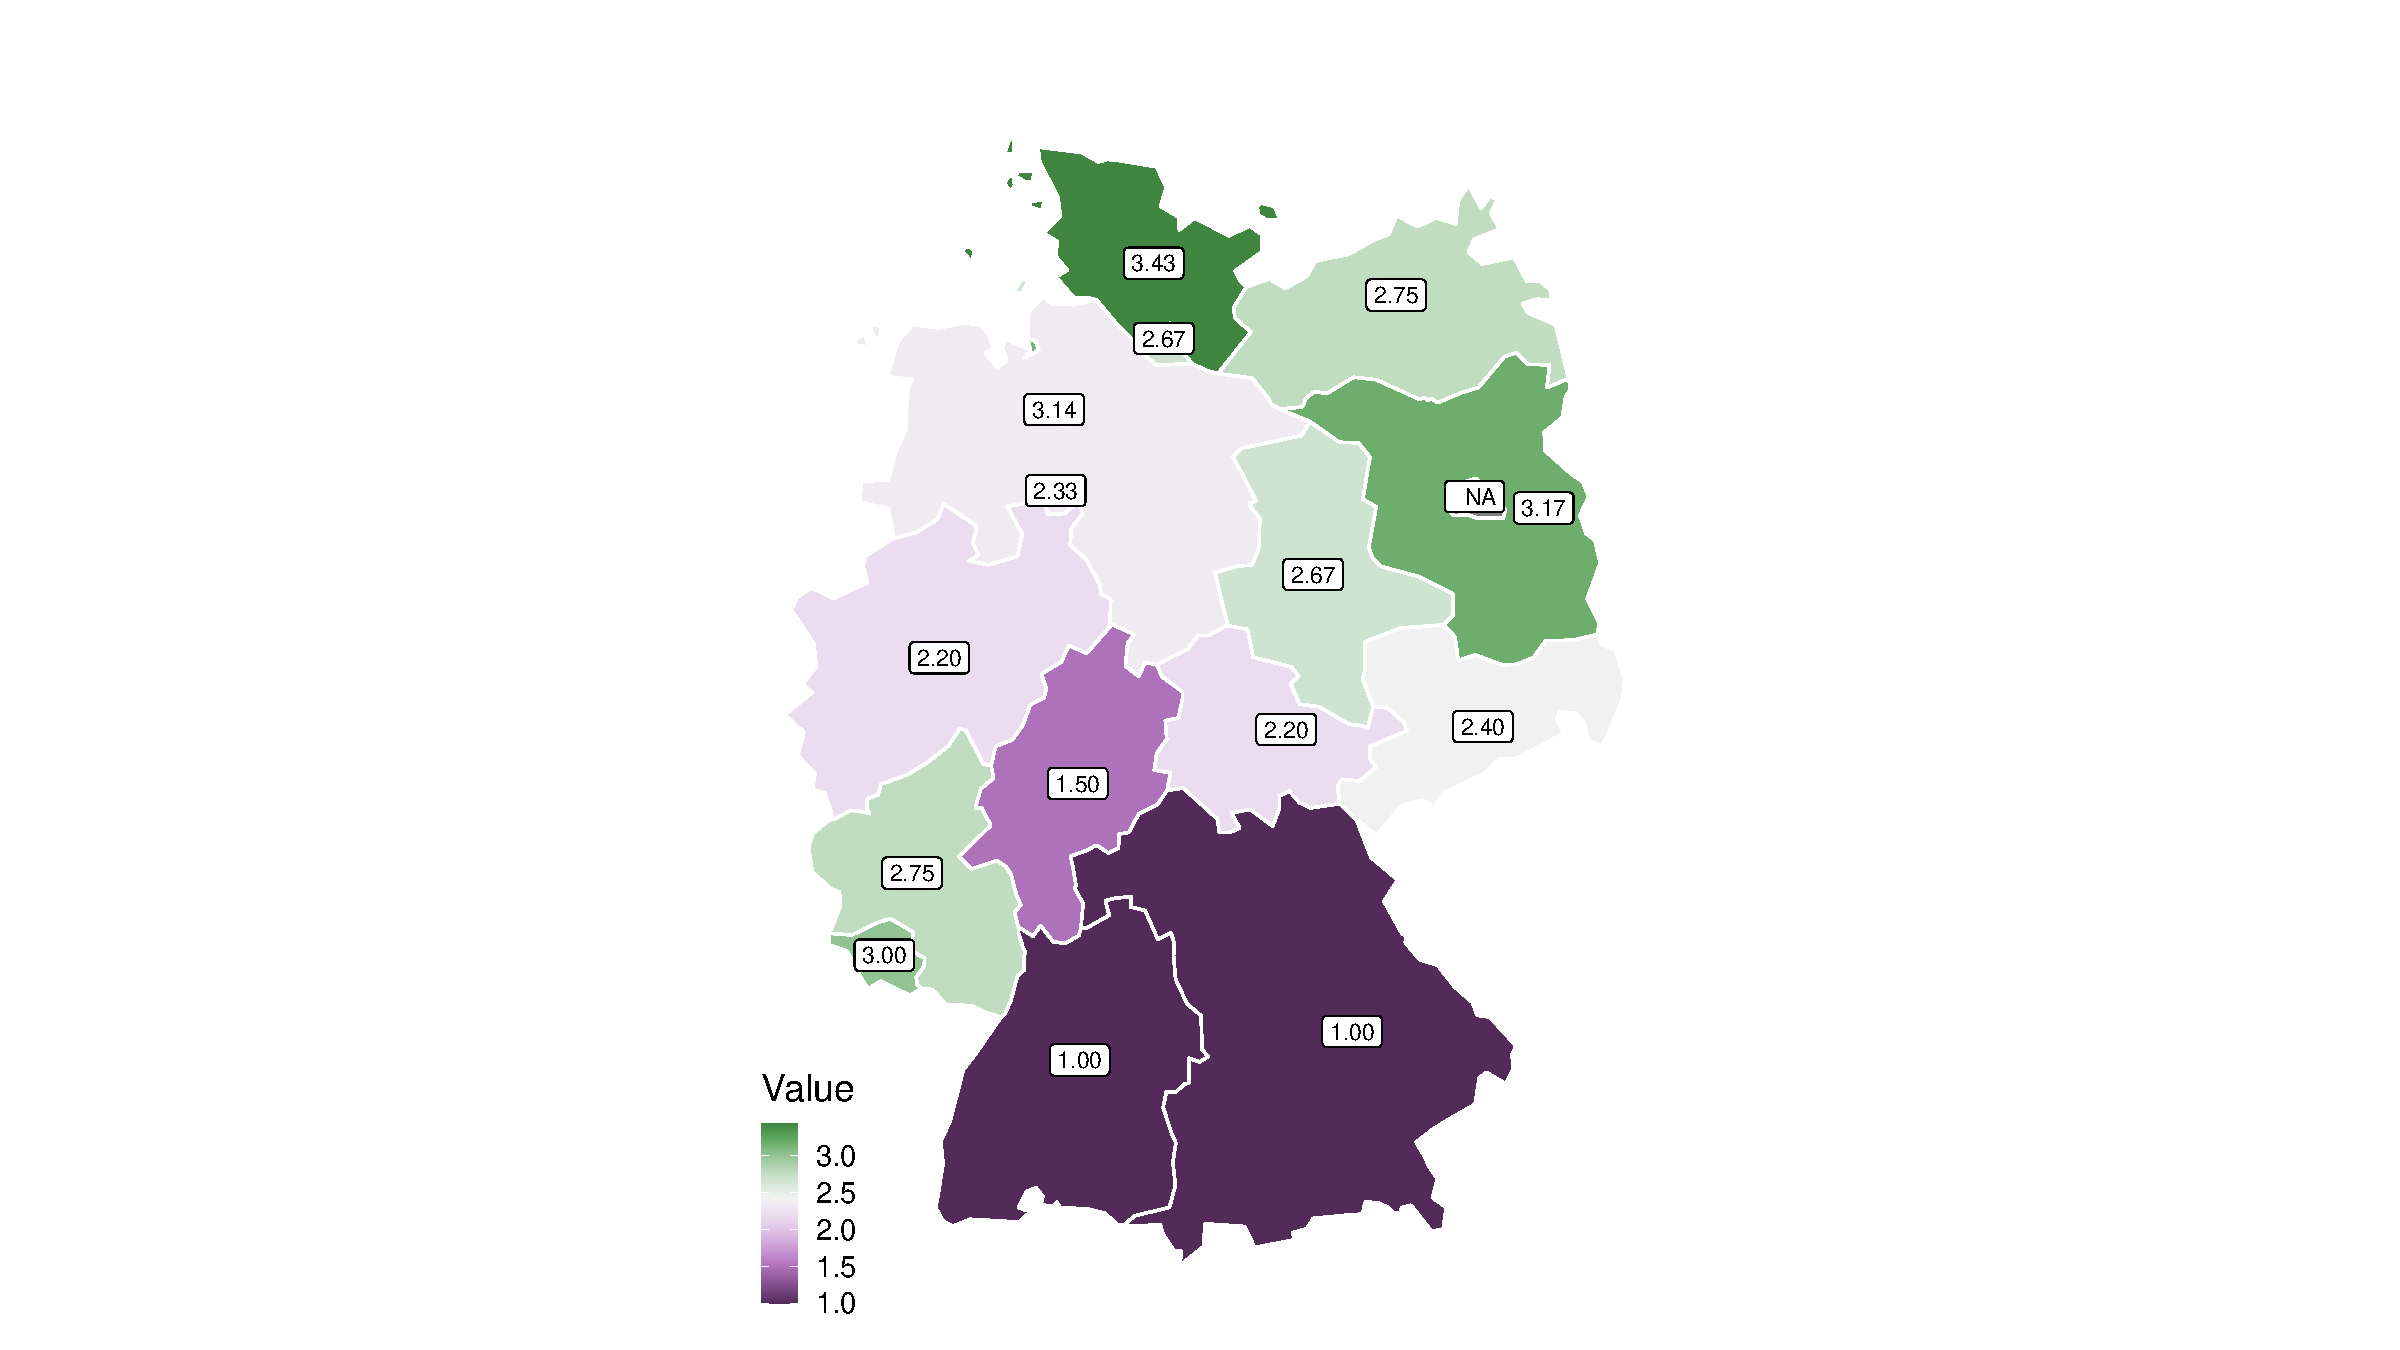
\includegraphics[width = \linewidth]{fedattAVG.pdf}
\caption{States' attitudes toward federalism (average values)}
\label{fig.attitudemap}
\end{figure}

The assignment of statements could potentially introduce bias due to the subjectivity of coders. To minimize this, we adopt a systematic data collection and transformation design. Several coders independently assess each passage according to predefined criteria, and we utilize Fleiss-$\kappa$ \citep{Fleiss2003} to evaluate the inter-rater reliability.\footnote{
	The Fleiss-$\kappa$ is a measure of inter-rater reliability, particularly suitable for cases with more than two raters, as in our study.
} The obtained Fleiss-$\kappa$ of 0.787 ($p$-value $=0.00$) indicates an almost perfect and highly significant inter-coder agreement.

The fact that attitudes towards federalism vary among the population and correspondingly within the respective state governments has been frequently addressed in the research literature. However, there are different explanatory approaches, all of which positively correlate with the data in Figure \ref{fig.attitudemap}.

Firstly, a growing body of literature identifies a link between contemporary attitudes towards federalism and Prussian history. Prussia dominated the German Empire and vigorously opposed Catholicism, which opposed the liberal and centralized state. These conflicts culminated in the so-called Kulturkampf. Haffert (2022) demonstrated that Catholics in regions affected by the Kulturkampf still maintain different political attitudes today compared to Catholics who were not directly affected by the Kulturkampf.